\documentclass[11pt,a4paper]{article}
\usepackage[T1]{fontenc}
\usepackage[utf8]{inputenc}
\usepackage{lmodern,microtype}
\usepackage[a4paper,margin=25mm,headheight=16pt,headsep=10pt]{geometry}
\usepackage{amsmath,amssymb,amsthm,mathtools,bm}
\usepackage{booktabs,tabularx,array,enumitem}
\usepackage{xcolor,hyperref,fancyhdr,lastpage}
\usepackage{tikz}
\usetikzlibrary{arrows.meta,positioning,calc}
\definecolor{ink}{HTML}{1B263B}
\definecolor{blue}{HTML}{205D8E}
\definecolor{light}{HTML}{E1E8F0}
\hypersetup{colorlinks=true,linkcolor=blue,urlcolor=blue,citecolor=blue,
  pdftitle={Spin and Symmetry in Quantum Mechanics: Complete Assignment V Consolidated Solutions},
  pdfauthor={Quantum Mechanics I Study Manuscript},
  pdfsubject={Stern--Gerlach, Pauli matrices, spin measurement, parity, translation and rotation symmetries}}
\setlength{\parindent}{0pt}
\setlength{\parskip}{5pt}
\setlength{\emergencystretch}{2.5em}
\allowdisplaybreaks[2]
\pagestyle{fancy}
\fancyhf{}
\fancyhead[L]{\small\sffamily QUANTUM MECHANICS I / ASSIGNMENT V}
\fancyhead[R]{\small\sffamily PARTS A + B: 25 SOLUTIONS}
\fancyfoot[L]{\footnotesize Educational mathematical-physics manuscript}
\fancyfoot[R]{\small\thepage\ / \pageref{LastPage}}
\renewcommand{\headrulewidth}{0.3pt}
\newtheorem{theorem}{Theorem}[section]
\newtheorem{proposition}[theorem]{Proposition}
\newtheorem{lemma}[theorem]{Lemma}
\theoremstyle{definition}
\newtheorem{remark}[theorem]{Remark}
\newcommand{\ket}[1]{\left|#1\right\rangle}
\newcommand{\bra}[1]{\left\langle#1\right|}
\newcommand{\avg}[1]{\left\langle #1\right\rangle}
\newcommand{\ip}[2]{\left\langle#1\middle|#2\right\rangle}
\newcommand{\HH}{\mathcal H}
\newcommand{\UU}{\hat U}
\newcommand{\PP}{\hat{\mathcal P}}
\newcommand{\grad}{\boldsymbol\nabla}
\newcommand{\result}[1]{\begin{center}\fcolorbox{light}{white}{\begin{minipage}{0.88\textwidth}\centering\vspace{2pt}\(\displaystyle #1\)\vspace{2pt}\end{minipage}}\end{center}}
\newenvironment{question}{\begin{quote}\small\noindent\textbf{Assignment question.}\ }{\end{quote}}
\newcommand{\exam}[1]{\par\medskip\noindent\textbf{Examination conclusion.}\ #1\par}
\begin{document}
\begin{titlepage}
\thispagestyle{empty}
\vspace*{18mm}
{\color{blue}\rule{\textwidth}{1.7pt}}\par\vspace{11mm}
{\LARGE\sffamily\bfseries Spin and Symmetry in Quantum Mechanics\par}
\vspace{5mm}
{\Large\sffamily Complete Consolidated Assignment V: Parts A and B\par}
\vspace{10mm}
{\large\bfseries Twenty-five rigorously worked problems in M.Sc. Quantum Mechanics--I\par}
\vspace{12mm}
\noindent\textbf{Topics:} Pauli matrix algebra and spin ladders; space and time translation generators; parity and inversion; polar and axial tensors; hydrogen wavefunction parity; Laporte selection rule; symmetry and degeneracy; Stern--Gerlach measurements; spinor probabilities and uncertainty; two-particle dynamics; angular-momentum conservation and rotational multiplets.
\vspace{12mm}
\begin{center}
\vspace{3mm}
{\large\color{blue}\(\displaystyle\sigma_j\sigma_k=\delta_{jk}I_2+i\varepsilon_{jkl}\sigma_l\quad\vert\quad[\hat H,\hat J_i]=0\)}
\vspace{3mm}
\end{center}
\vfill
\noindent\textbf{Source note:} The supplied \texttt{QM-AS-1-5.pdf} contains a page titled \emph{Assignment V--Part I} with four Part A and five Part B questions, plus a later, expanded block printed \emph{Assignment IV} with fifteen Part A and ten Part B questions. To honor the request for a \emph{complete consolidated set}, this manuscript includes all fifteen Part A and all ten Part B questions (25 total), clearly marking the source-label discrepancy rather than silently renumbering the original source.
\vspace{8mm}
\noindent\textbf{Status:} Pedagogical preprint, formatted in an arXiv-inspired \LaTeX{} article style. It is \emph{not} an arXiv submission and does not claim original research or peer review.
\vspace{9mm}
\noindent November 2026\par\vspace{6mm}
{\color{blue}\rule{\textwidth}{1.7pt}}
\end{titlepage}
\begin{abstract}
These notes give self-contained derivations for the consolidated set of fifteen Part A short-answer and ten Part B long-answer quantum mechanics questions (25 in all), drawn from two overlapping blocks of the supplied course assignment PDF. Calculations proceed from canonical commutation relations, Hilbert-space projection, and unitary symmetry operators: Pauli and ladder algebra, generators of spatial and temporal translations, parity and inversion, tensor transformation types, hydrogenic parity and electric-dipole selection rules, spin measurements, and conservation laws are proved explicitly. A two-particle harmonic interaction is separated into center-of-mass and relative degrees of freedom. The consequences of parity and continuous rotations are treated, including selection rules, conserved angular momentum, and the scope of rotational degeneracy. Assumptions, phase conventions and limits of the statements are stated explicitly. This is an instructional synthesis of coursework solutions, not a research claim.
\end{abstract}
\tableofcontents
\bigskip
\section*{Conventions and mathematical preliminaries}
\addcontentsline{toc}{section}{Conventions and mathematical preliminaries}
We use \(\hbar=h/(2\pi)\) and the physicists' inner product \(\ip{\phi}{\psi}\), conjugate-linear in the first slot. On \(L^2(\mathbb R^d)\), \(\hat p_i=-i\hbar\partial_i\); on the common suitable domains, \([\hat x_i,\hat p_j]=i\hbar\delta_{ij}\). Pauli matrices are \(\sigma_i\) and \(\hat S_i=\hbar\sigma_i/2\). For spinors we choose the ordered \(S_z\) basis \((\ket{+z},\ket{-z})\). All probability formulas assume normalized states, unless otherwise indicated. For spatial symmetries, \(\hat U(R)=e^{-i\theta\mathbf n\cdot\hat{\mathbf J}/\hbar}\) acts actively on states, with observables transforming in expectation by \(\hat U^\dagger\hat A\hat U\). Mathematical operator equalities involving unbounded quantities are understood on a suitable invariant dense domain.\par
\noindent\textbf{How to read this manuscript.} Each Part A or Part B section restates its source problem, develops the proof, discusses physical implications and qualifications, and ends with an examination-ready conclusion. The expanded source set has been used to avoid omitting related Part A or B problems.

\section*{Part A --- Short-answer problems: complete derivations}
\addcontentsline{toc}{section}{Part A --- Short-answer problems}
\noindent The expanded block in the supplied composite assignment file lists fifteen Part A questions. Questions A1--A4 also appear under the separately headed \emph{Assignment V--Part I}; A5--A15 appear in the expanded block printed under \emph{Assignment IV}. All fifteen are included to make the consolidated document self-contained.

\section{A1. Prove that the Pauli spin matrices are Hermitian and unitary}
\begin{question}Show that the Pauli spin matrices are both Hermitian and unitary.\end{question}
\subsection{Definitions and adjoints}
In the ordered spin-$z$ basis $\{\ket{+z},\ket{-z}\}$, the three Pauli matrices are
\begin{equation}
\sigma_x=\begin{pmatrix}0&1\\1&0\end{pmatrix},\quad
\sigma_y=\begin{pmatrix}0&-i\\i&0\end{pmatrix},\quad
\sigma_z=\begin{pmatrix}1&0\\0&-1\end{pmatrix}.
\label{eq:A-paulis}
\end{equation}
An operator $A$ is Hermitian if $A^\dagger=A$, where $\dagger$ means transpose followed by complex conjugation. Matrix-by-matrix,
\begin{align}
\sigma_x^\dagger&=\begin{pmatrix}0&1\\1&0\end{pmatrix}=\sigma_x,\\
\sigma_y^\dagger&=\left(\begin{pmatrix}0&-i\\i&0\end{pmatrix}^{*}\right)^{\mathsf T}
=\begin{pmatrix}0&-i\\i&0\end{pmatrix}=\sigma_y,\\
\sigma_z^\dagger&=\begin{pmatrix}1&0\\0&-1\end{pmatrix}=\sigma_z.
\end{align}
Thus every $\sigma_i$ is Hermitian. A matrix $U$ is unitary if $U^\dagger U=I$. Direct multiplication gives
\begin{align}
\sigma_x^2&=\begin{pmatrix}0&1\\1&0\end{pmatrix}^{2}=I_2,\\
\sigma_y^2&=\begin{pmatrix}0&-i\\i&0\end{pmatrix}^{2}
=\begin{pmatrix}(-i)i&0\\0&i(-i)\end{pmatrix}=I_2,\\
\sigma_z^2&=\begin{pmatrix}1&0\\0&-1\end{pmatrix}^{2}=I_2.
\end{align}
Since $\sigma_i^\dagger=\sigma_i$, it follows that $\sigma_i^\dagger\sigma_i=\sigma_i^2=I_2$. Hence
\result{\sigma_i^\dagger=\sigma_i,\qquad \sigma_i^\dagger\sigma_i=I_2,\quad i=x,y,z.}
\paragraph{Physical check.} Hermiticity ensures real spin-component eigenvalues; unitarity of $\sigma_i$ ensures preservation of the spinor norm under its action. Note that the physical spin operators $S_i=\hbar\sigma_i/2$ are Hermitian, but are \emph{not} unitary unless one introduces dimensionless normalization: $S_i^\dagger S_i=\hbar^2I_2/4$.
\exam{The Pauli matrices are Hermitian because $\sigma_i^\dagger=\sigma_i$ and unitary because $\sigma_i^2=I_2$, so $\sigma_i^\dagger\sigma_i=I_2$.}

\section{A2. Prove the Pauli-matrix product identity}
\begin{question}Show that $\sigma_j\sigma_k=\delta_{jk}I_2+i\sum_l\varepsilon_{jkl}\sigma_l$, where $j,k,l\in\{x,y,z\}$.\end{question}
The Pauli matrices in Eq.~\eqref{eq:A-paulis} have squares $\sigma_x^2=\sigma_y^2=\sigma_z^2=I_2$. This proves the identity for $j=k$, since $\delta_{jj}=1$ and $\varepsilon_{jjl}=0$.
For distinct indices, explicitly calculate
\begin{align}
\sigma_x\sigma_y&=\begin{pmatrix}i&0\\0&-i\end{pmatrix}=i\sigma_z,\\
\sigma_y\sigma_z&=\begin{pmatrix}0&i\\i&0\end{pmatrix}=i\sigma_x,\\
\sigma_z\sigma_x&=\begin{pmatrix}0&1\\-1&0\end{pmatrix}=i\sigma_y.
\end{align}
Reversing the order changes the sign:
\begin{equation}
\sigma_y\sigma_x=-i\sigma_z,\quad
\sigma_z\sigma_y=-i\sigma_x,\quad
\sigma_x\sigma_z=-i\sigma_y.
\end{equation}
For distinct $j,k$, precisely one $l$ makes $\varepsilon_{jkl}$ nonzero, and its sign records the order of multiplication. Combining the diagonal and off-diagonal cases yields
\result{\sigma_j\sigma_k=\delta_{jk}I_2+i\sum_{l=x,y,z}\varepsilon_{jkl}\sigma_l.}
Interchange $j$ and $k$ and add or subtract the two product identities:
\begin{align}
\{\sigma_j,\sigma_k\}&=\sigma_j\sigma_k+\sigma_k\sigma_j=2\delta_{jk}I_2,\label{eq:A-anti}\\
[\sigma_j,\sigma_k]&=\sigma_j\sigma_k-\sigma_k\sigma_j=2i\sum_l\varepsilon_{jkl}\sigma_l.\label{eq:A-sigcomm}
\end{align}
\paragraph{Conventions.} The identity contains the $2\times2$ identity $I_2$ multiplying $\delta_{jk}$; it is frequently suppressed typographically. Indices $j,k,l$ label spatial directions, not matrix entries.
\exam{The explicit cyclic products, reverse products, and squares exhaust all ordered pairs $(j,k)$, establishing the product rule and its commutator/anticommutator corollaries.}

\section{A3. Verify spin-component and ladder-operator commutators}
\begin{question}Using Pauli spin matrices, verify $[S_x,S_y]=i\hbar S_z$, $[S_z,S_\pm]=\pm\hbar S_\pm$, and $[S_+,S_-]=2\hbar S_z$.\end{question}
Define
\begin{equation}
S_i=\frac\hbar2\sigma_i,\quad
S_\pm=S_x\pm iS_y.
\end{equation}
Using the Pauli matrices,
\begin{equation}
S_+=\hbar\begin{pmatrix}0&1\\0&0\end{pmatrix},\qquad
S_-=\hbar\begin{pmatrix}0&0\\1&0\end{pmatrix},\qquad
S_z=\frac\hbar2\begin{pmatrix}1&0\\0&-1\end{pmatrix}.
\end{equation}
\subsection{First identity}
Equation~\eqref{eq:A-sigcomm} gives $[\sigma_x,\sigma_y]=2i\sigma_z$. Hence
\begin{equation}
[S_x,S_y]=\frac{\hbar^2}{4}[\sigma_x,\sigma_y]
=\frac{i\hbar^2}{2}\sigma_z=i\hbar S_z.
\end{equation}
\subsection{Second identity}
Direct multiplication yields
\begin{align}
S_zS_+&=\frac{\hbar^2}{2}\begin{pmatrix}0&1\\0&0\end{pmatrix},&
S_+S_z&=-\frac{\hbar^2}{2}\begin{pmatrix}0&1\\0&0\end{pmatrix},\\
S_zS_-&=-\frac{\hbar^2}{2}\begin{pmatrix}0&0\\1&0\end{pmatrix},&
S_-S_z&=\frac{\hbar^2}{2}\begin{pmatrix}0&0\\1&0\end{pmatrix}.
\end{align}
Subtracting each pair gives
\begin{equation}
[S_z,S_+]=\hbar S_+,\qquad [S_z,S_-]=-\hbar S_-.
\end{equation}
\subsection{Third identity}
Similarly,
\begin{equation}
S_+S_-=\hbar^2\begin{pmatrix}1&0\\0&0\end{pmatrix},\qquad
S_-S_+=\hbar^2\begin{pmatrix}0&0\\0&1\end{pmatrix}.
\end{equation}
Therefore,
\begin{equation}
[S_+,S_-]=\hbar^2\begin{pmatrix}1&0\\0&-1\end{pmatrix}=2\hbar S_z.
\end{equation}
\result{[S_x,S_y]=i\hbar S_z,\quad [S_z,S_\pm]=\pm\hbar S_\pm,\quad [S_+,S_-]=2\hbar S_z.}
\exam{All three commutators follow exactly from the Pauli algebra and the explicit $2\times2$ spin-$\frac12$ matrices.}

\section{A4. Prove that the spin ladder operators are not Hermitian}
\begin{question}Show that $\hat S_\pm$ are not Hermitian.\end{question}
By definition,
\begin{equation}
S_+=S_x+iS_y,\qquad S_-=S_x-iS_y.
\end{equation}
Since $S_x^\dagger=S_x$ and $S_y^\dagger=S_y$, and conjugation changes $i$ into $-i$,
\begin{align}
S_+^\dagger&=(S_x+iS_y)^\dagger=S_x-iS_y=S_-,\\
S_-^\dagger&=(S_x-iS_y)^\dagger=S_x+iS_y=S_+.
\end{align}
The operators are unequal. Explicitly,
\begin{equation}
S_+=\hbar\begin{pmatrix}0&1\\0&0\end{pmatrix},\quad
S_+^\dagger=\hbar\begin{pmatrix}0&0\\1&0\end{pmatrix}=S_-\ne S_+.
\end{equation}
Thus
\result{S_+^\dagger=S_-,\qquad S_-^\dagger=S_+,\qquad S_\pm^\dagger\ne S_\pm.}
\paragraph{Interpretation.} $S_+$ raises the $S_z$ magnetic quantum number, whereas $S_-$ lowers it. They are mutually adjoint rather than individually Hermitian. In contrast, $S_x=(S_++S_-)/2$ and $S_y=(S_+-S_-)/(2i)$ are Hermitian observables.
\exam{Neither $S_+$ nor $S_-$ equals its own adjoint; hence neither is Hermitian.}

\section{A5. Derive momentum as the generator of spatial translations}
\begin{question}Show that momentum is the generator of translations in space.\end{question}
For an active displacement by $a$ along $x$, a wavefunction transforms as
\begin{equation}
(T(a)\psi)(x)=\psi(x-a).
\label{eq:A-Tpsi}
\end{equation}
The minus sign is essential: a packet centered at $x_0$ is moved to $x_0+a$. Taylor expansion for infinitesimal $a$ gives
\begin{equation}
\psi(x-a)=\psi(x)-a\partial_x\psi(x)+O(a^2).
\end{equation}
In position representation $p_x=-i\hbar\partial_x$, so $\partial_x=(i/\hbar)p_x$. Therefore,
\begin{equation}
T(a)=I-\frac{ia}{\hbar}p_x+O(a^2).
\end{equation}
Composition of translations gives $T(a)T(b)=T(a+b)$ and, for the strongly continuous unitary family, the finite operator is
\result{T(a)=\exp\!\left(-\frac{ia}{\hbar}p_x\right).}
Its action is confirmed by the translation identity
\begin{equation}
e^{-a\partial_x}\psi(x)=\psi(x-a).
\end{equation}
For a vector displacement $\mathbf a$ and many particles, the generator of \emph{common} translation is the total momentum $\mathbf P=\sum_a\mathbf p_a$:
\begin{equation}
T(\mathbf a)=\exp[-i\mathbf a\cdot\mathbf P/\hbar].
\end{equation}
Because momentum is self-adjoint, $T(a)^\dagger T(a)=I$. The position shift can also be checked using Baker--Campbell--Hausdorff and $[x,p_x]=i\hbar$:
\begin{align}
T(a)^\dagger xT(a)&=e^{ia p_x/\hbar}xe^{-ia p_x/\hbar}=x+a,\\
T(a)^\dagger p_xT(a)&=p_x.
\end{align}
\paragraph{Symmetry consequence.} If $T(a)^\dagger HT(a)=H$ for every $a$, differentiation at $a=0$ gives $[H,p_x]=0$, so $d p_{x,H}/dt=0$ for a momentum operator with no explicit time dependence.
\exam{The coefficient of $-ia/\hbar$ in the infinitesimal unitary translation is $p_x$, proving that momentum generates translations.}

\section{A6. Derive the Hamiltonian as the generator of time translations}
\begin{question}Show that the Hamiltonian is the generator of translations in time.\end{question}
For a closed system with a time-independent self-adjoint Hamiltonian $H$, the Schr\"odinger equation is
\begin{equation}
i\hbar\frac{d}{dt}\ket{\psi(t)}=H\ket{\psi(t)}.
\end{equation}
Define the propagator by $\ket{\psi(t)}=U(t,t_0)\ket{\psi(t_0)}$, with $U(t_0,t_0)=I$. It satisfies
\begin{equation}
i\hbar\partial_t U(t,t_0)=H U(t,t_0).
\end{equation}
For constant $H$, the solution is
\result{U(t,t_0)=e^{-iH(t-t_0)/\hbar}.}
For a short increment $\delta t$,
\begin{equation}
U(t_0+\delta t,t_0)=I-\frac{i\delta t}{\hbar}H+O(\delta t^2).
\end{equation}
Thus $H$ is the infinitesimal generator of time translations, in exact analogy with the role of momentum for spatial translations. Self-adjointness implies
\begin{equation}
U(t,t_0)^\dagger U(t,t_0)=I,
\end{equation}
which preserves state norms. On an energy eigenstate $H\ket E=E\ket E$,
\begin{equation}
U(t,t_0)\ket E=e^{-iE(t-t_0)/\hbar}\ket E,
\end{equation}
so the energy determines the phase accumulated during time evolution.
\paragraph{Time-dependent qualification.} For $H(t)$ the short-time generator remains the instantaneous Hamiltonian, but one must generally use
\begin{equation}
U(t,t_0)=\mathcal T\exp\!\left[-\frac{i}{\hbar}\int_{t_0}^t H(s)\,ds\right],
\end{equation}
where $\mathcal T$ time-orders noncommuting Hamiltonians. A time-dependent Hamiltonian does not in general give a one-parameter group $e^{-iH\Delta t/\hbar}$ or energy conservation.
\exam{The first-order propagator is $I-iH\delta t/\hbar$, proving that $H$ generates infinitesimal time evolution.}

\section{A7. Define the parity operator and determine its eigenvalues}
\begin{question}Define parity operator. Find its eigenvalues.\end{question}
For a spinless position-space wavefunction on an inversion-invariant domain, parity (spatial inversion) is
\begin{equation}
(\PP\psi)(\mathbf r)=\psi(-\mathbf r).
\end{equation}
It is a linear operator. Applying it twice,
\begin{equation}
(\PP^2\psi)(\mathbf r)=\psi(-(-\mathbf r))=\psi(\mathbf r),
\end{equation}
so $\PP^2=I$. If $\PP\psi_\pi=\pi\psi_\pi$ for a nonzero eigenfunction, then
\begin{equation}
\psi_\pi=\PP^2\psi_\pi=\pi^2\psi_\pi
\quad\Longrightarrow\quad \pi^2=1.
\end{equation}
Therefore
\result{\pi=+1\ \text{(even)},\qquad\pi=-1\ \text{(odd)}.}
In one dimension, $\psi_+(-x)=\psi_+(x)$ and $\psi_-(-x)=-\psi_-(x)$. Every wavefunction decomposes as
\begin{equation}
\psi_\pm(x)=\frac12\left[\psi(x)\pm\psi(-x)\right],\qquad
\psi=\psi_++\psi_-,
\end{equation}
corresponding to orthogonal projectors $\Pi_\pm=(I\pm\PP)/2$.
\exam{Parity reverses all spatial coordinates and squares to identity, so its eigenvalues are exactly $\pm1$.}

\section{A8. Prove that parity is Hermitian and unitary}
\begin{question}Show that the parity operator is Hermitian and unitary.\end{question}
For normalized or square-integrable states $\phi,\psi$, consider the inner product
\begin{equation}
\ip{\PP\phi}{\PP\psi}=
\int_{\mathbb R^3}\phi^*(-\mathbf r)\psi(-\mathbf r)\,d^3r.
\end{equation}
Under $\mathbf u=-\mathbf r$, the absolute Jacobian is $1$, and the domain $\mathbb R^3$ is unchanged. Hence
\begin{equation}
\ip{\PP\phi}{\PP\psi}=\int_{\mathbb R^3}\phi^*(\mathbf u)\psi(\mathbf u)\,d^3u=\ip\phi\psi.
\end{equation}
Therefore $\PP^\dagger\PP=I$, proving unitarity and $\PP^\dagger=\PP^{-1}$. But, by direct action, $\PP^2=I$, so $\PP^{-1}=\PP$. Hence
\result{\PP^\dagger=\PP^{-1}=\PP,\qquad \PP^\dagger\PP=I.}
The operator is thus both Hermitian and unitary. Its eigenvalues $\pm1$ are real and lie on the unit circle, as these properties require.
\paragraph{Scope.} The proof assumes inversion maps the Hilbert space and physical boundary conditions to themselves. A general spinful state may also carry an intrinsic parity factor; this calculation concerns spatial inversion of the orbital wavefunction.
\exam{Norm preservation establishes unitarity; the involution $\PP^2=I$ then forces $\PP^\dagger=\PP$.}

\section{A9. Differentiate a true scalar from a pseudoscalar}
\begin{question}Differentiate between a true scalar and a pseudoscalar.\end{question}
Under a proper rotation $R\in SO(3)$, both a true scalar $A$ and a pseudoscalar $B$ are invariant:
\begin{equation}
A'=A,\qquad B'=B\qquad (\det R=+1).
\end{equation}
The difference appears under an improper orthogonal transformation $Q\in O(3)$ with $\det Q=-1$. A true scalar obeys
\begin{equation}
\boxed{A'=A}\qquad\text{for every }Q\in O(3),
\end{equation}
whereas a pseudoscalar obeys
\begin{equation}
\boxed{B'=(\det Q)B}.
\end{equation}
In particular, spatial inversion $Q=-I_3$ has $\det Q=-1$, so a true scalar is even and a pseudoscalar is odd:
\begin{equation}
A\mapsto A,\qquad B\mapsto-B.
\end{equation}
\paragraph{Examples.} $r^2=\mathbf r\cdot\mathbf r$ and $\mathbf p^2$ are true scalars. Helicity-type operators $\mathbf S\cdot\mathbf p$ are pseudoscalars, because $\mathbf S$ is axial (unchanged by parity) while $\mathbf p$ is polar (sign reversed). The triple product $\mathbf a\cdot(\mathbf b\times\mathbf c)$ of three polar vectors is a pseudoscalar.
\begin{center}\small\begin{tabular}{@{}lll@{}}\toprule
Quantity & Proper rotation & Spatial inversion\\\midrule
True scalar & Unchanged & Unchanged\\
Pseudoscalar & Unchanged & Changes sign\\\bottomrule
\end{tabular}\end{center}
\paragraph{Quantum form.} If $P$ is the parity operator, then $P^\dagger A P=A$ for a true scalar and $P^\dagger B P=-B$ for a pseudoscalar, while both commute with the generators of proper rotations if their domains permit.
\exam{A true scalar is even under inversion; a pseudoscalar is invariant under proper rotations but odd under inversion.}

\section{A10. Differentiate a true vector from a pseudovector}
\begin{question}Differentiate between a true vector and a pseudovector.\end{question}
Under proper rotations, both polar (true) and axial (pseudo) vectors transform in the same way. If $R\in SO(3)$,
\begin{equation}
\mathbf V'=R\mathbf V,\qquad\mathbf A'=R\mathbf A.
\end{equation}
For a general orthogonal transformation $Q\in O(3)$, the distinction is
\begin{equation}
\boxed{\mathbf V'=Q\mathbf V}\quad\text{(polar vector)},
\end{equation}
\begin{equation}
\boxed{\mathbf A'=(\det Q)Q\mathbf A}\quad\text{(axial vector)}.
\end{equation}
For inversion $Q=-I_3$, $\det Q=-1$. Consequently,
\begin{equation}
\boxed{\mathbf V\mapsto-\mathbf V,\qquad\mathbf A\mapsto+\mathbf A.}
\end{equation}
\paragraph{Examples.} Position, momentum, velocity and electric field are polar vectors; orbital angular momentum $\mathbf L=\mathbf r\times\mathbf p$, spin $\mathbf S$ and magnetic field are axial vectors. Indeed, under inversion $\mathbf r\mapsto-\mathbf r$ and $\mathbf p\mapsto-\mathbf p$, so $\mathbf L\mapsto(-\mathbf r)\times(-\mathbf p)=\mathbf L$.
\begin{center}\small\begin{tabular}{@{}lll@{}}\toprule
Quantity & Proper rotation & Spatial inversion\\\midrule
True (polar) vector & $R\mathbf V$ & $-\mathbf V$\\
Pseudo (axial) vector & $R\mathbf A$ & $+\mathbf A$\\\bottomrule
\end{tabular}\end{center}
\paragraph{Operator commutators.} Both kinds obey $[J_i,V_j]=i\hbar\varepsilon_{ijk}V_k$ under proper rotations; that test alone does not distinguish them. The distinction requires parity or another orientation-reversing transformation.
\exam{Polar and axial vectors transform identically under proper rotations, but with opposite intrinsic behavior under inversion.}

\section{A11. Show that hydrogenic angular-momentum eigenfunctions have parity $(-1)^l$}
\begin{question}Show that $\hat{\mathcal P}\,\psi_{nlm}(r,\theta,\phi)=(-1)^l\psi_{nlm}(r,\theta,\phi)$.\end{question}
In a central potential the orbital stationary states separate:
\begin{equation}
\psi_{nlm}(r,\theta,\phi)=R_{nl}(r)Y_l^m(\theta,\phi).
\end{equation}
Under inversion $\mathbf r\mapsto-\mathbf r$, spherical coordinates transform as
\begin{equation}
r\mapsto r,\qquad\theta\mapsto\pi-\theta,\qquad\phi\mapsto\phi+\pi.
\end{equation}
The radial factor is unchanged. Write the spherical harmonics schematically as
\begin{equation}
Y_l^m(\theta,\phi)=N_{lm}P_l^m(\cos\theta)e^{im\phi},
\end{equation}
with the usual convention extended to negative $m$. The associated Legendre parity identity is
\begin{equation}
P_l^m(-u)=(-1)^{l+m}P_l^m(u),
\end{equation}
and the azimuthal factor satisfies $e^{im(\phi+\pi)}=(-1)^m e^{im\phi}$ for integer $m$. Therefore,
\begin{align}
Y_l^m(\pi-\theta,\phi+\pi)
&=(-1)^{l+m}(-1)^mY_l^m(\theta,\phi)\\
&=(-1)^lY_l^m(\theta,\phi).
\end{align}
Consequently,
\begin{align}
(\PP\psi_{nlm})(r,\theta,\phi)
&=R_{nl}(r)Y_l^m(\pi-\theta,\phi+\pi)\\
&=(-1)^l\psi_{nlm}(r,\theta,\phi).
\end{align}
\result{\PP\psi_{nlm}=(-1)^l\psi_{nlm}.}
Thus $s,d,g,\ldots$ orbital states ($l$ even) have even orbital parity, and $p,f,\ldots$ ($l$ odd) have odd orbital parity. The result refers to the orbital spatial factor; intrinsic parity factors must be accounted for separately in a full multi-particle description.
\exam{Spherical harmonics acquire $(-1)^l$ under inversion while the radial function is unchanged.}

\section{A12. Derive Laporte's rule from parity}
\begin{question}Derive Laporte's rule.\end{question}
Let $H_0$ be an inversion-symmetric unperturbed Hamiltonian, $[H_0,\PP]=0$, and let the initial and final energy eigenstates have definite parity:
\begin{equation}
\PP\ket i=\pi_i\ket i,\qquad\PP\ket f=\pi_f\ket f,\qquad\pi_i,\pi_f=\pm1.
\end{equation}
The electric dipole operator is $\mathbf d=\sum_a q_a\mathbf r_a$. Being a polar vector, it is odd under inversion:
\begin{equation}
\PP^\dagger\mathbf d\PP=-\mathbf d.
\end{equation}
The electric-dipole transition amplitude is proportional to $\mathbf d_{fi}=\bra f\mathbf d\ket i$. Insert $I=\PP^\dagger\PP$ on both sides of $\mathbf d$:
\begin{align}
\mathbf d_{fi}
&=\bra f\PP^\dagger(\PP\mathbf d\PP^\dagger)\PP\ket i\\
&=\pi_f\pi_i(-1)\bra f\mathbf d\ket i\\
&=-\pi_f\pi_i\mathbf d_{fi}.
\end{align}
Thus $(1+\pi_f\pi_i)\mathbf d_{fi}=0$. For a nonzero electric-dipole matrix element,
\result{\pi_f\pi_i=-1\quad\Longleftrightarrow\quad\pi_f=-\pi_i.}
This is \emph{Laporte's rule}: for a centrosymmetric system, electric-dipole transitions are forbidden between states of the same parity ($g\leftrightarrow g$ or $u\leftrightarrow u$), and parity allows $g\leftrightarrow u$ transitions. The labels $g$ (gerade) and $u$ (ungerade) refer to even and odd inversion parity.
For a one-electron central potential $\pi=(-1)^l$, so parity requires $\Delta l$ odd; the angular momentum selection rules for an E1 photon further restrict the familiar single-electron case to $\Delta l=\pm1$ (with suitable magnetic quantum number conditions).
\paragraph{Limitation.} Opposite parity is a necessary, not sufficient, condition for a nonzero E1 amplitude. Magnetic-dipole or electric-quadrupole transitions, external parity breaking, or state mixing can permit processes forbidden in the pure E1 inversion-symmetric approximation.
\exam{Because the dipole operator is odd, its matrix element between equal-parity states vanishes; the E1 transition must change parity.}

\section{A13. Show that hydrogen's internal ground state has zero mean electron momentum}
\begin{question}Show that if the electron in the hydrogen atom is in the ground state, then necessarily $\avg{\mathbf p_e}=\mathbf0$.\end{question}
We take the standard nucleus-fixed (or internal relative-coordinate) hydrogen Hamiltonian and its normalized real $1s$ wavefunction,
\begin{equation}
\psi_{100}(\mathbf r)=\frac1{\sqrt{\pi a_0^3}}e^{-r/a_0},\quad r=|\mathbf r|,
\end{equation}
where $a_0$ is the Bohr radius for the chosen reduced-mass convention. The momentum operator is $\mathbf p=-i\hbar\grad$. Its mean is
\begin{equation}
\avg{\mathbf p}=\int_{\mathbb R^3}\psi_{100}^*(\mathbf r)(-i\hbar\grad)\psi_{100}(\mathbf r)\,d^3r.
\end{equation}
Because $\psi_{100}$ depends only on $r$,
\begin{equation}
\grad\psi_{100}=-\frac1{a_0}\psi_{100}\,\hat{\mathbf r}.
\end{equation}
Thus
\begin{equation}
\avg{\mathbf p}=\frac{i\hbar}{a_0}\int |\psi_{100}(r)|^2\hat{\mathbf r}\,d^3r.
\end{equation}
The angular integral of the radial unit vector vanishes by spherical symmetry,
\begin{equation}
\int_{S^2}\hat{\mathbf r}\,d\Omega=\mathbf0,
\end{equation}
so
\result{\avg{\mathbf p_e}=\mathbf0\qquad\text{(hydrogen internal ground state / nucleus-fixed frame)}.}
An independent symmetry proof uses parity. The $1s$ orbital has $l=0$, hence $\PP\ket{1s}=+\ket{1s}$, whereas $\PP\mathbf p\PP=-\mathbf p$. Therefore
\begin{equation}
\avg{\mathbf p}=\bra{1s}\PP\mathbf p\PP\ket{1s}=-\avg{\mathbf p},
\end{equation}
which forces $\avg{\mathbf p}=0$.
\paragraph{Physical qualification.} The phrase "electron momentum" refers here to internal/relative motion in the atomic rest frame or the conventional fixed-nucleus approximation. A freely moving hydrogen atom can have a nonzero center-of-mass momentum, so the laboratory electron momentum need not vanish merely because the atom is internally in its ground state.
\exam{The normalized $1s$ state is spherically symmetric and even under parity, while momentum is parity odd; its expectation value therefore vanishes.}

\section{A14. Show that $L_z$ generates rotations about the $z$-axis}
\begin{question}Show that $\hat L_z$ is the generator of rotations about the $z$-axis.\end{question}
In Cartesian coordinates the orbital angular momentum is
\begin{equation}
L_z=xp_y-yp_x=-i\hbar\left(x\partial_y-y\partial_x\right).
\end{equation}
Use $x=r\sin\theta\cos\phi$, $y=r\sin\theta\sin\phi$, so
\begin{equation}
\partial_\phi=-y\partial_x+x\partial_y.
\end{equation}
Hence
\result{L_z=-i\hbar\frac{\partial}{\partial\phi}.}
An active rotation by angle $\alpha$ about the $z$ axis carries the wavefunction according to
\begin{equation}
(U_z(\alpha)\psi)(r,\theta,\phi)=\psi(r,\theta,\phi-\alpha).
\end{equation}
For small $\alpha$, Taylor expansion gives
\begin{equation}
\psi(\phi-\alpha)=\psi(\phi)-\alpha\partial_\phi\psi(\phi)+O(\alpha^2).
\end{equation}
Substitute $\partial_\phi=(i/\hbar)L_z$:
\begin{equation}
U_z(\alpha)=I-\frac{i\alpha}{\hbar}L_z+O(\alpha^2).
\end{equation}
Finite rotations follow by exponentiation:
\result{U_z(\alpha)=\exp\!\left(-\frac{i\alpha}{\hbar}L_z\right).}
The Heisenberg action confirms the geometric rotation. Since $[L_z,x]=i\hbar y$ and $[L_z,y]=-i\hbar x$,
\begin{align}
U_z^\dagger(\alpha)xU_z(\alpha)&=x\cos\alpha-y\sin\alpha,\\
U_z^\dagger(\alpha)yU_z(\alpha)&=x\sin\alpha+y\cos\alpha.
\end{align}
For eigenfunctions $e^{im\phi}$, $L_ze^{im\phi}=m\hbar e^{im\phi}$, and a rotation multiplies the state by $e^{-im\alpha}$.
\exam{The coefficient of $-i\alpha/\hbar$ in the infinitesimal $z$-rotation operator is $L_z$, establishing it as the generator.}

\section{A15. Explain the connection between symmetry and degeneracy}
\begin{question}Explain the connection between symmetry and degeneracy in brief.\end{question}
Let $U(g)$ be a unitary symmetry of a Hamiltonian $H$, so
\begin{equation}
U(g)^\dagger HU(g)=H\quad\Longleftrightarrow\quad[H,U(g)]=0.
\end{equation}
Suppose $H\ket{E,\alpha}=E\ket{E,\alpha}$. Then
\begin{equation}
H\bigl(U(g)\ket{E,\alpha}\bigr)
=U(g)H\ket{E,\alpha}
=E\bigl(U(g)\ket{E,\alpha}\bigr).
\end{equation}
Therefore every symmetry operation maps an energy eigenstate into the \emph{same energy eigenspace}. If the transformed state is linearly independent of the original state, a degeneracy follows. If it is merely proportional, no degeneracy is forced.
For full rotational invariance,
\begin{equation}
[H,J_x]=[H,J_y]=[H,J_z]=0,
\end{equation}
so $[H,J_\pm]=0$. The ladder formula
\begin{equation}
J_\pm\ket{j,m}=\hbar\sqrt{(j\mp m)(j\pm m+1)}\ket{j,m\pm1}
\end{equation}
connects states of the same energy with $m=-j,-j+1,\ldots,j$. One irreducible multiplet therefore has
\result{g_j=2j+1.}
\paragraph{Caveats.} A symmetry does not automatically generate degeneracy: parity has only one-dimensional irreducible representations, and the inversion-symmetric one-dimensional harmonic oscillator has nondegenerate bound-state levels. Similarly, $j=0$ is a rotational singlet. Further "accidental" degeneracies can arise from extra dynamical symmetries, such as the Runge--Lenz symmetry of the Coulomb problem; an external field can break full rotational symmetry and split a multiplet.
\exam{A symmetry preserves energy eigenspaces. Degeneracy is enforced when a multidimensional irreducible representation of the symmetry acts within an energy eigenspace, as with the $2j+1$ magnetic states of a rotation multiplet.}

\clearpage
\section*{Part B --- Long-answer problems}
\addcontentsline{toc}{section}{Part B --- Long-answer problems}

\section{B1. Space quantization and the Stern--Gerlach experiment}
\begin{question}Explain space quantization using the results of the Stern--Gerlach experiment.\end{question}
\subsection{Physical construction}
A collimated beam of neutral silver atoms crosses a spatially nonuniform magnetic field and then strikes a detection screen. The atoms are neutral, so the essential separation arises from the magnetic dipole interaction rather than the Lorentz force on a charged beam. For an atom carrying a magnetic moment \(\hat{\bm\mu}\), the interaction Hamiltonian in an external field is
\begin{equation}
\hat H_{\rm int}=-\hat{\bm\mu}\cdot\mathbf B(\mathbf r).
\label{eq:SGH}
\end{equation}
The corresponding force is \(\hat{\mathbf F}=-\grad\hat H_{\rm int}=\grad(\hat{\bm\mu}\cdot\mathbf B)\). If the field is predominantly along \(z\) and has a gradient \(G=\partial B_z/\partial z\), then under the usual approximation
\begin{equation}
\hat F_z\simeq\hat\mu_z\,G.
\end{equation}
For an electron, \(\hat{\bm\mu}_s=-g_s\mu_B\hat{\mathbf S}/\hbar\), with \(\mu_B=e\hbar/(2m_e)\) and \(g_s\simeq2\). A spin-\(\frac12\) state has \(S_z\)-eigenvalues \(\pm\hbar/2\), and therefore two magnetic-moment eigenvalues \(\mp g_s\mu_B/2\). The field gradient produces two opposite deflections rather than a continuous distribution. For the ground-state silver atom the dominant unpaired-electron contribution is effectively spin one-half, while the full atomic magnetic moment also includes atomic-structure details.
\begin{center}
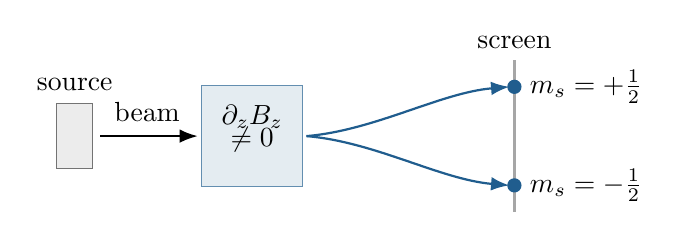
\begin{tikzpicture}[scale=.92,>=Latex]
\draw[fill=gray!15,draw=black!55] (-3,-.45) rectangle (-2.5,.45);\node[above] at (-2.75,.5){source};
\draw[->,thick] (-2.4,0)--(-1.05,0);\node[above] at (-1.75,0.07){beam};
\draw[fill=blue!12,draw=blue!70] (-1,-.7) rectangle (.4,.7);\node at (-.3,.27){\(\partial_zB_z\)};\node at (-.3,-.05){\(\neq0\)};
\draw[->,thick,blue] (.45,.0) .. controls (1.4,.08) and (2.3,.6) .. (3.25,.68);
\draw[->,thick,blue] (.45,.0) .. controls (1.4,-.08) and (2.3,-.6) .. (3.25,-.68);
\draw[gray!70,thick] (3.32,-1.05)--(3.32,1.05);
\fill[blue] (3.32,.68) circle (2.8pt);\fill[blue] (3.32,-.68) circle (2.8pt);
\node[right] at (3.4,.68){\(m_s=+\tfrac12\)};
\node[right] at (3.4,-.68){\(m_s=-\tfrac12\)};
\node[above] at (3.32,1.07){screen};
\end{tikzpicture}
\end{center}
\subsection{Measurement amplitudes and space quantization}
In the \(z\)-spin basis an arbitrary normalized spinor is \(\ket\psi=a\ket{+z}+b\ket{-z}\), where \(|a|^2+|b|^2=1\). Initially the spin and spatial motion can be prepared independently. During the magnet interaction they become correlated:
\begin{equation}
\ket\Psi\ \longrightarrow\ a\ket{\phi_+}\ket{+z}+b\ket{\phi_-}\ket{-z},
\end{equation}
where \(\ket{\phi_\pm}\) describe oppositely displaced outgoing wavepackets (their labels depend on field orientation and the magnetic-moment sign). When the packets are well resolved on the detector, the probabilities for the two branches obey the Born rule:
\begin{equation}
\boxed{P_+=|\ip{+z}{\psi}|^2=|a|^2,\qquad P_-=|b|^2,\qquad P_++P_-=1.}
\end{equation}
The observable projection is discrete even though the deflection distance is a continuous spatial coordinate. A hypothetical classical dipole with arbitrary orientation would suggest a continuous range of projections, whereas the measured resolved outcomes select discrete spin projections. The experiment is thus evidence for \emph{space quantization} and, in the silver-atom setting, two effective spin branches.
\exam{A nonuniform magnetic field spatially separates \(\hat S_z\)-eigencomponents with eigenvalues \(\pm\hbar/2\). The two outcomes, with Born probabilities \(|a|^2\) and \(|b|^2\), demonstrate quantization of the component of intrinsic angular momentum along the chosen measurement axis.}

\section{B2. Spin matrices in the \(\hat S^2,\hat S_z\) eigenbasis}
\begin{question}Construct the spin matrices for an electron using the eigenbasis of \(\hat S^2\) and \(\hat S_z\).\end{question}
\subsection{Basis and ladder algebra}
For an electron \(s=\tfrac12\), with the ordered orthonormal basis
\begin{equation}
\ket+\equiv\ket{\tfrac12,\tfrac12}=\begin{pmatrix}1\\0\end{pmatrix},\quad
\ket-\equiv\ket{\tfrac12,-\tfrac12}=\begin{pmatrix}0\\1\end{pmatrix},
\end{equation}
we have \(\hat S^2\ket{s,m}=\hbar^2s(s+1)\ket{s,m}\) and \(\hat S_z\ket{s,m}=\hbar m\ket{s,m}\). Hence
\begin{equation}
\hat S^2=\frac{3\hbar^2}{4}I_2,\qquad
\hat S_z=\frac\hbar2\begin{pmatrix}1&0\\0&-1\end{pmatrix}.
\end{equation}
Define \(\hat S_\pm=\hat S_x\pm i\hat S_y\). Angular momentum theory gives
\begin{equation}
\hat S_\pm\ket{s,m}=\hbar\sqrt{s(s+1)-m(m\pm1)}\ket{s,m\pm1}.
\end{equation}
For \(s=\frac12\), the coefficient is \(\sqrt{3/4-(-1/4)}=1\) on the nonzero steps, so
\begin{equation}
\hat S_+\ket-=\hbar\ket+ ,\quad \hat S_+\ket+=0,\quad
\hat S_-\ket+=\hbar\ket-,\quad \hat S_-\ket-=0.
\end{equation}
Reading off columns yields
\begin{equation}
\hat S_+=\hbar\begin{pmatrix}0&1\\0&0\end{pmatrix},\qquad
\hat S_-=\hbar\begin{pmatrix}0&0\\1&0\end{pmatrix}.
\end{equation}
Since \(\hat S_x=(\hat S_++\hat S_-)/2\) and \(\hat S_y=(\hat S_+-\hat S_-)/(2i)\), we obtain
\begin{equation}
\boxed{\begin{aligned}
\hat S_x&=\frac\hbar2\begin{pmatrix}0&1\\1&0\end{pmatrix},&
\hat S_y&=\frac\hbar2\begin{pmatrix}0&-i\\i&0\end{pmatrix},&
\hat S_z&=\frac\hbar2\begin{pmatrix}1&0\\0&-1\end{pmatrix}.
\end{aligned}}
\label{eq:spinmats}
\end{equation}
These are \(\hat S_i=(\hbar/2)\sigma_i\), with the three Pauli matrices \(\sigma_i\).
\subsection{Checks}
The matrices are Hermitian, \(\hat S_i^\dagger=\hat S_i\). Direct multiplication gives
\begin{equation}
[\hat S_x,\hat S_y]=\frac{\hbar^2}{4}[\sigma_x,\sigma_y]
=\frac{\hbar^2}{4}(2i\sigma_z)=i\hbar\hat S_z,
\end{equation}
with cyclic analogues. Each \(\sigma_i^2=I_2\), so
\begin{equation}
\hat S^2=\sum_i\hat S_i^2=3\frac{\hbar^2}{4}I_2,
\end{equation}
consistent with \(s(s+1)\hbar^2=3\hbar^2/4\).
\exam{In the \(\ket{s=\frac12,m=\pm\frac12}\) basis, the spin matrices are exactly \(\hat S_i=\hbar\sigma_i/2\); the ladder construction fixes all off-diagonal entries, and the commutator and Casimir checks validate the result.}

\section{B3. Eigenvalues and normalized eigenvectors of the Pauli matrices}
\begin{question}Determine the eigenvalues and the normalized eigenvectors of the Pauli spin matrices.\end{question}
All Pauli matrices are Hermitian and satisfy \(\sigma_i^2=I_2\). The eigenvalue problem is \(\sigma_i v=\lambda v\). We explicitly evaluate each characteristic polynomial and solve the linear systems.
\subsection{Matrix \(\sigma_x\)}
\begin{equation}
\det(\sigma_x-\lambda I)=\begin{vmatrix}-\lambda&1\\1&-\lambda\end{vmatrix}=\lambda^2-1.
\end{equation}
Thus \(\lambda=\pm1\). At \(\lambda=+1\), the system \(-a+b=0\), \(a-b=0\) gives \(b=a\); norm \(2|a|^2=1\) permits \(a=1/\sqrt2\). At \(\lambda=-1\), \(a+b=0\) gives \(b=-a\). Therefore
\begin{equation}
\boxed{\ket{+x}=\frac1{\sqrt2}\begin{pmatrix}1\\1\end{pmatrix},\qquad
\ket{-x}=\frac1{\sqrt2}\begin{pmatrix}1\\-1\end{pmatrix}.}
\end{equation}
\subsection{Matrix \(\sigma_y\)}
\begin{equation}
\det(\sigma_y-\lambda I)=\begin{vmatrix}-\lambda&-i\\i&-\lambda\end{vmatrix}
=\lambda^2-(-i)i=\lambda^2-1.
\end{equation}
For \(\lambda=+1\), \(-a-ib=0\), i.e. \(b=ia\). For \(\lambda=-1\), \(a-ib=0\), i.e. \(b=-ia\). Normalizing gives
\begin{equation}
\boxed{\ket{+y}=\frac1{\sqrt2}\begin{pmatrix}1\\i\end{pmatrix},\qquad
\ket{-y}=\frac1{\sqrt2}\begin{pmatrix}1\\-i\end{pmatrix}.}
\end{equation}
\subsection{Matrix \(\sigma_z\)}
\begin{equation}
\det(\sigma_z-\lambda I)=\begin{vmatrix}1-\lambda&0\\0&-1-\lambda\end{vmatrix}
=\lambda^2-1.
\end{equation}
For \(\lambda=+1\), the second component vanishes; for \(\lambda=-1\), the first vanishes:
\begin{equation}
\boxed{\ket{+z}=\begin{pmatrix}1\\0\end{pmatrix},\qquad
\ket{-z}=\begin{pmatrix}0\\1\end{pmatrix}.}
\end{equation}
\subsection{Orthogonality, projectors, completeness, and phases}
For each \(i=x,y,z\), verify \(\ip{+i}{+i}=\ip{-i}{-i}=1\) and \(\ip{+i}{-i}=0\). For example, \(\ip{+y}{-y}=\frac12(1+(-i)(-i))=0\). Let \(\Pi_{i,\pm}=\ket{\pm i}\bra{\pm i}\). Direct multiplication gives
\begin{align}
\Pi_{x,\pm}&=\frac12\begin{pmatrix}1&\pm1\\\pm1&1\end{pmatrix},&
\Pi_{y,\pm}&=\frac12\begin{pmatrix}1&\mp i\\\pm i&1\end{pmatrix},\\
\Pi_{z,+}&=\begin{pmatrix}1&0\\0&0\end{pmatrix},&
\Pi_{z,-}&=\begin{pmatrix}0&0\\0&1\end{pmatrix}.
\end{align}
Thus \(\Pi_{i,+}+\Pi_{i,-}=I_2\), \(\Pi_{i,+}\Pi_{i,-}=0\), and \(\Pi_{i,\pm}^2=\Pi_{i,\pm}=\Pi_{i,\pm}^\dagger\). The spectral decompositions are
\begin{equation}
\boxed{\sigma_i=\Pi_{i,+}-\Pi_{i,-},\qquad \Pi_{i,\pm}=\frac{I_2\pm\sigma_i}{2}.}
\end{equation}
Multiplying any eigenvector by \(e^{i\chi}\) preserves its norm, eigenvalue and projector: this is the physically irrelevant global phase freedom of a single eigenket. The eigenvalues of \(\hat S_i=\hbar\sigma_i/2\) are \(\pm\hbar/2\).
\exam{Each Pauli matrix has characteristic polynomial \(\lambda^2-1\) and eigenvalues \(\pm1\). The above six kets are normalized orthogonal eigenbases; their projectors sum to the identity and yield the spectral resolutions \(\sigma_i=\Pi_{i,+}-\Pi_{i,-}\).}

\section{B4. Expansion of an arbitrary spinor in three eigenbases}
\begin{question}For \(\ket\psi=(a,b)^{\mathsf T}\), express the electron spin state as a linear combination of eigenvectors of (i) \(\hat S_z\), (ii) \(\hat S_x\), and (iii) \(\hat S_y\).\end{question}
Assume \(a,b\in\mathbb C\) and \(|a|^2+|b|^2=1\). For an orthonormal basis \(\{\ket{u_+},\ket{u_-}\}\), completeness is \(I=\ket{u_+}\bra{u_+}+\ket{u_-}\bra{u_-}\). Hence
\begin{equation}
\ket\psi=\ip{u_+}{\psi}\ket{u_+}+\ip{u_-}{\psi}\ket{u_-}.
\end{equation}
The coefficients are inner-product projection amplitudes, and their squared moduli are measurement probabilities.
\subsection{\(S_z\) basis}
Using \(\bra{+z}=(1,0)\) and \(\bra{-z}=(0,1)\),
\begin{equation}
\boxed{\ket\psi=a\ket{+z}+b\ket{-z}.}
\end{equation}
Reconstruction: \(a(1,0)^{\mathsf T}+b(0,1)^{\mathsf T}=(a,b)^{\mathsf T}\). The probabilities are \(P(z,+)=|a|^2\) and \(P(z,-)=|b|^2\).
\subsection{\(S_x\) basis}
Projection gives
\begin{align}
c_{x,+}&=\ip{+x}{\psi}=\frac{a+b}{\sqrt2},&
c_{x,-}&=\ip{-x}{\psi}=\frac{a-b}{\sqrt2}.
\end{align}
Therefore
\begin{equation}
\boxed{\ket\psi=\frac{a+b}{\sqrt2}\ket{+x}+\frac{a-b}{\sqrt2}\ket{-x}.}
\end{equation}
To reconstruct explicitly,
\begin{equation}
\frac12\left[(a+b)\begin{pmatrix}1\\1\end{pmatrix}+(a-b)\begin{pmatrix}1\\-1\end{pmatrix}\right]
=\begin{pmatrix}a\\b\end{pmatrix}.
\end{equation}
The probabilities are
\begin{equation}
\boxed{P(x,\pm)=\frac{|a\pm b|^2}{2};\quad P(x,+)+P(x,-)=|a|^2+|b|^2=1.}
\end{equation}
\subsection{\(S_y\) basis}
Conjugating the eigenkets is essential: \(\bra{+y}=(1,-i)/\sqrt2\), \(\bra{-y}=(1,i)/\sqrt2\). Thus
\begin{align}
c_{y,+}&=\ip{+y}{\psi}=\frac{a-ib}{\sqrt2},&
c_{y,-}&=\ip{-y}{\psi}=\frac{a+ib}{\sqrt2}.
\end{align}
Therefore
\begin{equation}
\boxed{\ket\psi=\frac{a-ib}{\sqrt2}\ket{+y}+\frac{a+ib}{\sqrt2}\ket{-y}.}
\end{equation}
Reconstructing,
\begin{equation}
\frac12\left[(a-ib)\begin{pmatrix}1\\i\end{pmatrix}+(a+ib)\begin{pmatrix}1\\-i\end{pmatrix}\right]
=\begin{pmatrix}a\\b\end{pmatrix}.
\end{equation}
The probabilities are \(P(y,+)=|a-ib|^2/2\) and \(P(y,-)=|a+ib|^2/2\), whose sum is one.
\subsection{Unitary basis changes}
The matrices whose columns are the eigenvectors are
\begin{equation}
U_x=\frac1{\sqrt2}\begin{pmatrix}1&1\\1&-1\end{pmatrix},\qquad
U_y=\frac1{\sqrt2}\begin{pmatrix}1&1\\i&-i\end{pmatrix}.
\end{equation}
Both satisfy \(U_i^\dagger U_i=I_2\). With \([\psi]_z=(a,b)^{\mathsf T}\), the coefficient columns are \([\psi]_x=U_x^\dagger[\psi]_z\) and \([\psi]_y=U_y^\dagger[\psi]_z\). Unitarity preserves the norm, proving the probability identities without separate expansion.
\exam{All three expansions follow from \(c_{i,\pm}=\ip{\pm i}{\psi}\). Their reconstruction and probability normalization confirm that each basis describes the identical state, not three different physical preparations.}

\section{B5. Normalization, spin probabilities, means, and uncertainties}
\begin{question}For the electron spinor \(\ket\psi=A(3i,4)^{\mathsf T}\): (i) normalize it; (ii)--(iv) find probabilities for \(S_z,S_x,S_y=\pm\hbar/2\); (v) calculate their expectation values; (vi) their standard deviations; (vii) verify \(\Delta S_x\Delta S_y\ge\frac\hbar2|\avg{S_z}|\).\end{question}
\subsection{Normalization and global phase}
The bra is \(\bra\psi=A^*(-3i,4)\), so
\begin{equation}
1=\ip\psi\psi=|A|^2[(-3i)(3i)+16]=25|A|^2.
\end{equation}
Therefore \(|A|=1/5\); the general choice is \(A=e^{i\chi}/5\), where \(\chi\in\mathbb R\) is a global phase. We choose \(A=1/5\):
\begin{equation}
\boxed{\ket\psi=\frac15\begin{pmatrix}3i\\4\end{pmatrix},\qquad
\bra\psi=\frac15(-3i,4),\qquad\ip\psi\psi=1.}
\label{eq:given-spinor}
\end{equation}
\subsection{Born probabilities along three axes}
Projection onto the normalized eigenvectors from Sec.~3 gives the six amplitudes
\begin{align}
\ip{+z}\psi&=\frac{3i}{5}, & \ip{-z}\psi&=\frac45,\\
\ip{+x}\psi&=\frac{4+3i}{5\sqrt2},& \ip{-x}\psi&=\frac{-4+3i}{5\sqrt2},\\
\ip{+y}\psi&=\frac{-i}{5\sqrt2},& \ip{-y}\psi&=\frac{7i}{5\sqrt2}.
\end{align}
Taking squared moduli gives
\begin{equation}
\boxed{\begin{array}{c|cc|c}
\text{Measurement}&P(+\hbar/2)&P(-\hbar/2)&\text{Sum}\\\hline
S_z&9/25&16/25&1\\ S_x&1/2&1/2&1\\ S_y&1/50&49/50&1
\end{array}}
\label{eq:probtable}
\end{equation}
For instance \(|4+3i|^2=25\), hence \(P(S_x=+\hbar/2)=25/50=1/2\); for the positive \(y\)-outcome the minus sign in \(\bra{+y}=(1,-i)/\sqrt2\) yields \(P=|-i/(5\sqrt2)|^2=1/50\). All probability rows sum to unity.
\subsection{Expectation values by matrix multiplication and Born averages}
Using \(\hat S_i=\hbar\sigma_i/2\),
\begin{align}
\avg{\hat S_x}&=\frac{\hbar}{50}(-3i,4)\begin{pmatrix}4\\3i\end{pmatrix}=0,\\
\avg{\hat S_y}&=\frac{\hbar}{50}(-3i,4)\begin{pmatrix}-4i\\-3\end{pmatrix}=-\frac{12\hbar}{25},\\
\avg{\hat S_z}&=\frac{\hbar}{50}(-3i,4)\begin{pmatrix}3i\\-4\end{pmatrix}=-\frac{7\hbar}{50}.
\end{align}
The Born-rule check is \(\avg{S_i}=\frac\hbar2(P_{i,+}-P_{i,-})\), producing exactly the same values. Thus
\begin{equation}
\boxed{\avg{\hat{\mathbf S}}=\left(0,-\frac{12\hbar}{25},-\frac{7\hbar}{50}\right).}
\end{equation}
\subsection{Uncertainties}
Since \(\sigma_i^2=I_2\), for every normalized spinor \(\avg{S_i^2}=\hbar^2/4\). The standard deviation is
\begin{equation}
(\Delta S_i)^2=\avg{S_i^2}-\avg{S_i}^2.
\end{equation}
Consequently,
\begin{align}
(\Delta S_x)^2&=\frac{\hbar^2}{4},\\
(\Delta S_y)^2&=\frac{\hbar^2}{4}-\frac{144\hbar^2}{625}=\frac{49\hbar^2}{2500},\\
(\Delta S_z)^2&=\frac{\hbar^2}{4}-\frac{49\hbar^2}{2500}=\frac{576\hbar^2}{2500}.
\end{align}
Thus
\begin{equation}
\boxed{\Delta S_x=\frac\hbar2,\qquad\Delta S_y=\frac{7\hbar}{50},\qquad\Delta S_z=\frac{12\hbar}{25}.}
\end{equation}
\subsection{Uncertainty relation and independent checks}
From \([\hat S_x,\hat S_y]=i\hbar\hat S_z\), the Robertson bound is \(\Delta S_x\Delta S_y\ge\frac\hbar2|\avg{S_z}|\). For the given spinor,
\begin{equation}
\underbrace{\Delta S_x\Delta S_y}_{\text{left side}}=\frac\hbar2\frac{7\hbar}{50}
=\frac{7\hbar^2}{100}
=\underbrace{\frac\hbar2\left|-\frac{7\hbar}{50}\right|}_{\text{right side}}.
\end{equation}
The state \emph{saturates} this bound. Its Bloch vector is \(\mathbf s=2\avg{\mathbf S}/\hbar=(0,-24/25,-7/25)\), and \(|\mathbf s|^2=(576+49)/625=1\), an independent pure-spinor check. The Schr\"odinger--Robertson covariance term vanishes here because \(\{S_x,S_y\}=0\) and \(\avg{S_x}=0\).
\exam{The normalized state is \((3i,4)^{\mathsf T}/5\); all six probabilities are in Eq.~\eqref{eq:probtable}. The means are \((0,-12\hbar/25,-7\hbar/50)\), the standard deviations are \((\hbar/2,7\hbar/50,12\hbar/25)\), and the \(x\)-\(y\) Robertson inequality holds at equality.}

\section{B6. Translational invariance and conservation of momentum}
\begin{question}Show that momentum is conserved if the Hamiltonian of a system is invariant under spatial translations.\end{question}
\subsection{Momentum generates translations}
In one dimension a positive physical displacement \(a\) acts on a wavefunction according to \((\UU(a)\psi)(x)=\psi(x-a)\). For infinitesimal \(a\), Taylor's theorem gives
\begin{equation}
\psi(x-a)=\psi(x)-a\partial_x\psi(x)+O(a^2)
=\left(I-\frac{ia}{\hbar}\hat p\right)\psi(x)+O(a^2),
\end{equation}
because \(\hat p=-i\hbar\partial_x\). Composition of infinitesimal displacements produces the unitary finite translation operator
\begin{equation}
\boxed{\UU(a)=e^{-ia\hat p/\hbar},\qquad \UU^\dagger(a)=\UU(-a).}
\end{equation}
For a simultaneous displacement of an isolated \(N\)-particle system, the generator is total momentum \(\hat{\mathbf P}=\sum_{\alpha=1}^N\hat{\mathbf p}_\alpha\), giving \(\UU(\mathbf a)=e^{-i\mathbf a\cdot\hat{\mathbf P}/\hbar}\). Translation by the same \(\mathbf a\) leaves all relative separations invariant.
\subsection{Infinitesimal symmetry proof}
Translation invariance along \(x\) means
\begin{equation}
\UU^\dagger(a)\hat H\UU(a)=\hat H\qquad\text{for every real }a.
\label{eq:translation-symmetry}
\end{equation}
Expand \(\UU(a)=I-ia\hat P_x/\hbar+O(a^2)\) and its adjoint. Then
\begin{align}
\UU^\dagger\hat H\UU
&=\left(I+\frac{ia}{\hbar}\hat P_x\right)\hat H
\left(I-\frac{ia}{\hbar}\hat P_x\right)+O(a^2)\\
&=\hat H+\frac{ia}{\hbar}(\hat P_x\hat H-\hat H\hat P_x)+O(a^2).
\end{align}
Because Eq.~\eqref{eq:translation-symmetry} holds at every \(a\), its coefficient linear in \(a\) must vanish:
\begin{equation}
\boxed{[\hat H,\hat P_x]=0.}
\end{equation}
Repeat along \(y\) and \(z\). Full spatial translation invariance yields
\begin{equation}
\boxed{[\hat H,\hat P_i]=0\ (i=x,y,z).}
\end{equation}
\subsection{Heisenberg equation and Ehrenfest theorem}
For an observable without explicit time dependence,
\begin{equation}
\frac{d\hat A_H}{dt}=\frac{i}{\hbar}[\hat H_H,\hat A_H].
\end{equation}
With \(\hat A=\hat P_i\), the vanishing commutator gives
\begin{equation}
\boxed{\frac{d\hat P_{i,H}}{dt}=0,\qquad\frac{d}{dt}\avg{\hat P_i}=0.}
\end{equation}
This holds for every state in the physical domain, whether or not the state is a momentum eigenstate. The entire momentum spectral distribution is invariant when the symmetry commutes with time evolution.
\subsection{Explicit force-law check}
For \(\hat H=\hat{\mathbf p}^{\,2}/(2m)+V(\hat{\mathbf r})\), on smooth test wavefunctions
\begin{align}
[V,\hat p_x]\psi
&=V(-i\hbar\partial_x\psi)+i\hbar\partial_x(V\psi)
=i\hbar(\partial_xV)\psi.
\end{align}
Thus \([\hat H,\hat p_i]=i\hbar\partial_iV\) and
\begin{equation}
\boxed{\frac{d\hat p_{i,H}}{dt}=-(\partial_i V)_H,\qquad
\frac{d}{dt}\avg{\hat p_i}=-\avg{\partial_iV}.}
\end{equation}
For full translation invariance, \(V(\mathbf r+\mathbf a)=V(\mathbf r)\) for arbitrary \(\mathbf a\), hence \(\grad V=0\) for a differentiable potential. For translation invariance only along \(x\), merely \(\partial_xV=0\) is needed to conserve \(p_x\). In an interacting system, relative potentials can be nonconstant even though total momentum remains conserved; one must then use \(\hat{\mathbf P}\), not any individual \(\hat{\mathbf p}_\alpha\).
\exam{Continuous translation invariance implies \([\hat H,\hat P_i]=0\) by differentiation of \(\UU^\dagger\hat H\UU=\hat H\) at the identity; the Heisenberg equation then proves \(d\hat P_{i,H}/dt=0\). This is the quantum translation--momentum conservation statement associated with Noether's theorem.}

\section{B7. Two particles coupled by a quadratic relative potential}
\begin{question}For particles of masses \(m_1,m_2\) in one dimension with \(\hat H=\hat p_1^2/(2m_1)+\hat p_2^2/(2m_2)+\frac k2(\hat x_1-\hat x_2)^2\), prove that \(\hat P=\hat p_1+\hat p_2\) is conserved.\end{question}
\subsection{Direct canonical commutator proof}
Assume \([\hat x_i,\hat p_j]=i\hbar\delta_{ij}\), \([\hat x_i,\hat x_j]=[\hat p_i,\hat p_j]=0\). Set \(\hat r=\hat x_1-\hat x_2\) and \(\hat P=\hat p_1+\hat p_2\). Then
\begin{align}
[\hat r,\hat p_1]&=i\hbar,& [\hat r,\hat p_2]&=-i\hbar,\\
[\hat r,\hat P]&=[\hat r,\hat p_1]+[\hat r,\hat p_2]=0.
\end{align}
The product rule \([A^2,B]=A[A,B]+[A,B]A\) yields \([\hat r^2,\hat P]=0\). Since all momenta commute,
\begin{equation}
\left[\frac{\hat p_1^2}{2m_1}+\frac{\hat p_2^2}{2m_2},\hat P\right]=0.
\end{equation}
Consequently,
\begin{equation}
\boxed{[\hat H,\hat P]=\frac{k}{2}[\hat r^2,\hat P]=0,\qquad
\frac{d\hat P_H}{dt}=\frac{i}{\hbar}[\hat H_H,\hat P_H]=0.}
\label{eq:2particle-conserve}
\end{equation}
\subsection{Internal forces}
In the Heisenberg picture,
\begin{align}
\dot{\hat p}_{1,H}&=\frac{i}{\hbar}[\hat H_H,\hat p_{1,H}]=-k(\hat x_{1,H}-\hat x_{2,H}),\\
\dot{\hat p}_{2,H}&=\frac{i}{\hbar}[\hat H_H,\hat p_{2,H}]=+k(\hat x_{1,H}-\hat x_{2,H}).
\end{align}
Here the interaction commutators are \([k\hat r^2/2,\hat p_1]=i\hbar k\hat r\) and \([k\hat r^2/2,\hat p_2]=-i\hbar k\hat r\). The internal forces cancel exactly, \(\dot{\hat p}_{1,H}+\dot{\hat p}_{2,H}=0\). Individual momenta vary, while their sum is conserved.
\subsection{Canonical center-of-mass transformation}
Define total and reduced masses
\begin{equation}
M=m_1+m_2,\qquad \mu=\frac{m_1m_2}{M},\qquad \frac1\mu=\frac1{m_1}+\frac1{m_2},
\end{equation}
and operators
\begin{align}
\hat R&=\frac{m_1\hat x_1+m_2\hat x_2}{M}, & \hat r&=\hat x_1-\hat x_2,\\
\hat P&=\hat p_1+\hat p_2, & \hat p&=\frac{m_2\hat p_1-m_1\hat p_2}{M}.
\label{eq:com}
\end{align}
Check each canonical commutator directly:
\begin{align}
[\hat R,\hat P]
&=\frac{m_1}{M}[\hat x_1,\hat p_1]+\frac{m_2}{M}[\hat x_2,\hat p_2]
=i\hbar,\\
[\hat r,\hat p]
&=\frac{m_2}{M}[\hat x_1,\hat p_1]+\frac{m_1}{M}[\hat x_2,\hat p_2]
=i\hbar,\\
[\hat R,\hat p]
&=\frac{m_1m_2}{M^2}[\hat x_1,\hat p_1]
-\frac{m_1m_2}{M^2}[\hat x_2,\hat p_2]=0,\\
[\hat r,\hat P]&=i\hbar-i\hbar=0.
\end{align}
The remaining commutators \([\hat R,\hat r]\) and \([\hat P,\hat p]\) vanish because all original positions commute, and all original momenta commute. Thus \((\hat R,\hat P)\) and \((\hat r,\hat p)\) are independent canonical pairs.
\subsection{Inverse transformation and kinetic energy}
Solving Eq.~\eqref{eq:com} yields
\begin{align}
\hat x_1&=\hat R+\frac{m_2}{M}\hat r,&\hat x_2&=\hat R-\frac{m_1}{M}\hat r,\\
\hat p_1&=\frac{m_1}{M}\hat P+\hat p,&\hat p_2&=\frac{m_2}{M}\hat P-\hat p.
\end{align}
Substitute into the kinetic energy. Since \([\hat P,\hat p]=0\), we may expand normally:
\begin{align}
\frac{\hat p_1^2}{2m_1}&=\frac{m_1}{2M^2}\hat P^2+\frac1M\hat P\hat p+\frac{\hat p^2}{2m_1},\\
\frac{\hat p_2^2}{2m_2}&=\frac{m_2}{2M^2}\hat P^2-\frac1M\hat P\hat p+\frac{\hat p^2}{2m_2}.
\end{align}
The mixed terms cancel, and we obtain
\begin{equation}
\boxed{\hat H=\underbrace{\frac{\hat P^2}{2M}}_{\hat H_{\rm CM}}
+\underbrace{\left(\frac{\hat p^2}{2\mu}+\frac{k}{2}\hat r^2\right)}_{\hat H_{\rm rel}}.}
\label{eq:separate}
\end{equation}
Because \([\hat P,\hat r]=[\hat P,\hat p]=0\), the center-of-mass and relative Hamiltonians commute. The center-of-mass coordinate obeys \(\dot{\hat R}_H=\hat P_H/M\), \(\ddot{\hat R}_H=0\). The relative equations are \(\dot{\hat r}_H=\hat p_H/\mu\), \(\dot{\hat p}_H=-k\hat r_H\), so
\begin{equation}
\ddot{\hat r}_H+\omega^2\hat r_H=0,\qquad \omega=\sqrt{k/\mu}\quad(k>0).
\end{equation}
For \(k>0\), the relative subsystem is a one-dimensional harmonic oscillator, with \(E_{{\rm rel},n}=\hbar\omega(n+\frac12)\). The total generalized stationary energies are
\begin{equation}
\boxed{E_{P,n}=\frac{P^2}{2M}+\hbar\sqrt{\frac{k}{\mu}}\left(n+\frac12\right).}
\end{equation}
On the whole line, a definite-\(P\) plane wave is delta-normalized rather than square-integrable; normalized wavepackets can be used for the center-of-mass sector. The linear coordinate transformation has Jacobian determinant \(-1\), so \(dx_1\,dx_2=dR\,dr\) and no extra factor appears in the norm. The frequency result assumes a stable \(k>0\) oscillator, whereas the conservation proof is valid for any real \(k\).
\exam{The total momentum \(\hat P\) commutes with the Hamiltonian because the relative coordinate commutes with \(\hat P\). The center-of-mass transformation proves this independently and splits the problem into a free center of mass and a harmonic internal mode.}

\section{B8. Inversion symmetry and parity consequences}
\begin{question}Explain inversion symmetry of a Hamiltonian and its consequences.\end{question}
\subsection{Definition, parity square, and self-adjointness}
Spatial inversion is \(\mathbf r\mapsto-\mathbf r\). The unitary parity operator \(\PP\) is defined on position wavefunctions by
\begin{equation}
\boxed{(\PP\psi)(\mathbf r)=\psi(-\mathbf r).}
\end{equation}
Twice applied, \((\PP^2\psi)(\mathbf r)=\psi(\mathbf r)\); therefore \(\PP^2=I\) and \(\PP^{-1}=\PP\). It preserves inner products:
\begin{equation}
\ip{\PP\phi}{\PP\psi}=\int d^3r\,\phi^*(-\mathbf r)\psi(-\mathbf r)
=\int d^3u\,\phi^*(\mathbf u)\psi(\mathbf u)=\ip\phi\psi.
\end{equation}
Thus \(\PP^\dagger\PP=I\), and together with \(\PP^{-1}=\PP\),
\begin{equation}
\boxed{\PP^2=I,\qquad \PP^\dagger=\PP^{-1}=\PP.}
\end{equation}
For a nonzero parity eigenstate \(\PP\ket\psi=\pi\ket\psi\), we have \(\pi^2=1\); hence \(\pi=\pm1\). Even and odd wavefunctions satisfy \(\psi_+(-\mathbf r)=\psi_+(\mathbf r)\), \(\psi_-(-\mathbf r)=-\psi_-(\mathbf r)\), respectively.
\subsection{Transformation of observables and Hamiltonian}
Applying \(\PP\) on either side of position and momentum yields
\begin{equation}
\boxed{\PP\hat{\mathbf r}\PP=-\hat{\mathbf r},\qquad
\PP\hat{\mathbf p}\PP=-\hat{\mathbf p}.}
\end{equation}
For example, in one dimension, \((\PP\hat x\PP\psi)(x)=-x\psi(x)\). For momentum, the chain rule gives \(-i\hbar\partial_x\psi(-x)=+i\hbar\psi'(-x)\), and the outer parity then yields \(-\hat p\psi(x)\). Squared momentum is even, while \(\hat{\mathbf L}=\hat{\mathbf r}\times\hat{\mathbf p}\) is axial and unchanged under parity. Spin is also axial under ordinary inversion.

For \(\hat H=\hat{\mathbf p}^{\,2}/(2m)+V(\hat{\mathbf r})\), assuming an inversion-symmetric operator domain,
\begin{equation}
\PP\hat H\PP=\frac{\hat{\mathbf p}^{\,2}}{2m}+V(-\hat{\mathbf r}).
\end{equation}
Hence the sufficient and, for this model, necessary symmetry criterion is \(V(-\mathbf r)=V(\mathbf r)\). Under this condition
\begin{equation}
\boxed{\PP^\dagger\hat H\PP=\hat H\quad\Longleftrightarrow\quad[\hat H,\PP]=0.}
\label{eq:parity}
\end{equation}
\subsection{Conservation and simultaneous eigenstates}
If \([\hat H,\PP]=0\) and \(\PP\) has no explicit time dependence, then \(d\PP_H/dt=(i/\hbar)[\hat H_H,\PP_H]=0\). Thus the probabilities for even and odd parity are conserved. Furthermore, if \(\hat H\ket E=E\ket E\), then \(\hat H(\PP\ket E)=E(\PP\ket E)\). If the energy level is nondegenerate, \(\PP\ket E=\pm\ket E\). In a degenerate eigenspace, one may choose an orthonormal simultaneous eigenbasis of \(\hat H\) and \(\PP\), although arbitrary superpositions of opposite parity at the same energy need not have definite parity.
\subsection{Parity projectors and selection rule}
The spectral projectors are
\begin{equation}
\boxed{\Pi_\pm=\frac{I\pm\PP}{2},\qquad\Pi_\pm^2=\Pi_\pm,\quad\Pi_+\Pi_-=0,\quad\Pi_++\Pi_-=I.}
\end{equation}
For a state \(\psi\), they produce \(\psi_\pm(\mathbf r)=[\psi(\mathbf r)\pm\psi(-\mathbf r)]/2\). If an operator \(\hat O\) has parity \(\eta_O\), meaning \(\PP\hat O\PP=\eta_O\hat O\), and initial and final eigenstates have parity \(\pi_i,\pi_f\), then
\begin{equation}
\ip{f}{\hat O\ket i}=\pi_f\pi_i\eta_O\,\ip{f}{\hat O\ket i},
\end{equation}
and therefore
\begin{equation}
\boxed{(1-\pi_f\pi_i\eta_O)\,\bra f\hat O\ket i=0.}
\end{equation}
A nonzero matrix element requires \(\pi_f\pi_i\eta_O=1\). In particular, the electric-dipole operator \(\hat{\mathbf d}=q\hat{\mathbf r}\) is odd, so an E1 transition requires opposite initial/final parities. Such a parity condition is necessary, not sufficient: angular momentum and other selection rules may additionally restrict transitions.
\subsection{Vanishing odd expectations, examples and degeneracy caveat}
For any definite-parity state and parity-odd observable \(\hat O\), \(\avg O=-\avg O\), hence \(\avg O=0\). In particular \(\avg{\mathbf r}=\avg{\mathbf p}=0\) when these expectations exist. For the 1D harmonic oscillator \(V(x)=m\omega^2x^2/2\), \(\psi_n(-x)=(-1)^n\psi_n(x)\); for hydrogenic central-potential states, \(Y_l^m(-\hat{\mathbf r})=(-1)^lY_l^m(\hat{\mathbf r})\). Parity alone does \emph{not} force energy degeneracy: the group \(\mathbb Z_2\) has one-dimensional irreducible representations, and the 1D oscillator is a concrete nondegenerate parity-invariant example.
\exam{Inversion symmetry is \(\PP^\dagger\hat H\PP=\hat H\) or \([\hat H,\PP]=0\). Since \(\PP^2=I\), its eigenvalues are \(\pm1\). Parity is conserved, permits even/odd symmetry-adapted eigenstates and imposes selection rules; degeneracy is not required by inversion symmetry alone.}

\section{B9. Scalar and vector operators under rotations}
\begin{question}Distinguish between a scalar operator and a vector operator on the basis of rotations.\end{question}
\subsection{Rotation convention and scalar law}
For proper spatial rotation \(R\in SO(3)\), states transform actively by \(\UU(R)=e^{-i\theta\mathbf n\cdot\hat{\mathbf J}/\hbar}\). A rotational scalar \(\hat A\) obeys
\begin{equation}
\boxed{\UU^\dagger(R)\hat A\UU(R)=\hat A.}
\end{equation}
For an infinitesimal rotation about axis \(i\), \(\UU=I-id\theta\hat J_i/\hbar+O(d\theta^2)\), \(\UU^\dagger=I+id\theta\hat J_i/\hbar+O(d\theta^2)\), giving
\begin{equation}
\UU^\dagger\hat A\UU=\hat A+\frac{id\theta}{\hbar}[\hat J_i,\hat A]+O(d\theta^2).
\end{equation}
Scalar invariance implies
\begin{equation}
\boxed{[\hat J_i,\hat A]=0\quad(i=x,y,z).}
\label{eq:scalar}
\end{equation}
Examples include \(\hat{\mathbf r}^{\,2}\), \(\hat{\mathbf p}^{\,2}\), \(\hat{\mathbf J}^{\,2}\), and \(\hat{\mathbf L}\cdot\hat{\mathbf S}\) under rotations generated by total angular momentum.
\subsection{Finite vector law and infinitesimal derivation}
A Cartesian vector operator \(\hat{\mathbf V}=(\hat V_x,\hat V_y,\hat V_z)\) satisfies
\begin{equation}
\boxed{\UU^\dagger(R)\hat V_i\UU(R)=\sum_jR_{ij}\hat V_j.}
\label{eq:vector-finite}
\end{equation}
For a rotation by \(d\theta\) about \(z\), the geometric law yields
\begin{equation}
\hat V_x'=\hat V_x-d\theta\hat V_y,\quad
\hat V_y'=\hat V_y+d\theta\hat V_x,\quad
\hat V_z'=\hat V_z.
\end{equation}
On the other hand, the unitary expansion gives \(\hat V_j'=\hat V_j+(id\theta/\hbar)[\hat J_z,\hat V_j]\). Comparing the two gives
\begin{equation}
\boxed{[\hat J_z,\hat V_x]=i\hbar\hat V_y,\quad
[\hat J_z,\hat V_y]=-i\hbar\hat V_x,\quad[\hat J_z,\hat V_z]=0.}
\end{equation}
For an infinitesimal rotation about arbitrary \(\mathbf n\), geometric variation is \(\delta\hat V_j=d\theta\sum_{i,k}\varepsilon_{jik}n_i\hat V_k\), while the unitary expansion is \(\delta\hat V_j=(id\theta/\hbar)\sum_i n_i[\hat J_i,\hat V_j]\). Since \(\mathbf n\) is arbitrary, and \(\varepsilon_{jik}=-\varepsilon_{ijk}\), the defining commutator follows:
\begin{equation}
\boxed{[\hat J_i,\hat V_j]=i\hbar\sum_k\varepsilon_{ijk}\hat V_k.}
\label{eq:vector-comm}
\end{equation}
\subsection{Canonical verification with position and momentum}
For a spinless particle, \(\hat L_i=\sum_{a,b}\varepsilon_{iab}\hat x_a\hat p_b\). Then
\begin{align}
[\hat L_i,\hat x_j]
&=\sum_{a,b}\varepsilon_{iab}\hat x_a[\hat p_b,\hat x_j]
=-i\hbar\sum_a\varepsilon_{iaj}\hat x_a
=i\hbar\sum_k\varepsilon_{ijk}\hat x_k,\\
[\hat L_i,\hat p_j]
&=\sum_{a,b}\varepsilon_{iab}[\hat x_a,\hat p_j]\hat p_b
=i\hbar\sum_k\varepsilon_{ijk}\hat p_k.
\end{align}
Thus position and momentum are vector operators. For a scalar example,
\begin{equation}
[\hat L_i,\hat{\mathbf r}^{\,2}]
=i\hbar\sum_{j,k}\varepsilon_{ijk}(\hat x_k\hat x_j+\hat x_j\hat x_k)=0
\end{equation}
because the parenthesized factor is symmetric in \(j,k\), while \(\varepsilon_{ijk}\) is antisymmetric.
\subsection{Spin--orbit scalar and spherical tensors}
Both \(\hat{\mathbf L}\) and \(\hat{\mathbf S}\) transform as vectors under total rotations generated by \(\hat{\mathbf J}=\hat{\mathbf L}+\hat{\mathbf S}\). Their dot product commutes with each \(\hat J_i\):
\begin{equation}
[\hat J_i,\hat{\mathbf L}\cdot\hat{\mathbf S}]
=i\hbar\sum_{j,k}\varepsilon_{ijk}(\hat L_k\hat S_j+\hat L_j\hat S_k)=0.
\end{equation}
A scalar is a rank-0 irreducible spherical tensor, while a vector is rank 1 with spherical components
\begin{equation}
T^{(1)}_{+1}=-\frac{V_x+iV_y}{\sqrt2},\qquad
T^{(1)}_0=V_z,\qquad
T^{(1)}_{-1}=\frac{V_x-iV_y}{\sqrt2}.
\end{equation}
These obey \([J_z,T^{(1)}_q]=\hbar qT^{(1)}_q\) and \([J_\pm,T^{(1)}_q]=\hbar\sqrt{(1\mp q)(1\pm q+1)}\,T^{(1)}_{q\pm1}\). Under proper rotations, polar vectors (\(\mathbf r,\mathbf p\)) and axial vectors (\(\mathbf L,\mathbf S\)) obey the same rank-1 law; they differ under inversion.
\begin{center}\small
\begin{tabularx}{.96\textwidth}{@{}p{.20\textwidth}XX@{}}\toprule
Property & Scalar \(A\) & Vector \(\mathbf V\) \\ \midrule
Finite rotations & \(U^\dagger AU=A\) & \(U^\dagger V_iU=R_{ij}V_j\)\\
Generators & \([J_i,A]=0\) & \([J_i,V_j]=i\hbar\varepsilon_{ijk}V_k\)\\
Tensor rank & \(k=0\), one component & \(k=1\), three Cartesian components\\
Examples & \(r^2,p^2,J^2,\mathbf L\cdot\mathbf S\) & \(\mathbf r,\mathbf p,\mathbf L,\mathbf S\)\\\bottomrule
\end{tabularx}
\end{center}
\exam{The definitive test is the commutator with generators: \([J_i,A]=0\) for a scalar and \([J_i,V_j]=i\hbar\varepsilon_{ijk}V_k\) for a vector. These are the rank-0 and rank-1 tensor representations of proper rotations.}

\section{B10. Continuous rotational symmetry and its consequences}
\begin{question}What is meant by continuous rotational symmetry of a Hamiltonian? What are its consequences?\end{question}
\subsection{Full rotation invariance implies generator commutators}
The Hamiltonian has full continuous rotational symmetry if
\begin{equation}
\boxed{\UU^\dagger(R)\hat H\UU(R)=\hat H\quad\text{for all }R\in SO(3),}
\label{eq:rotinv}
\end{equation}
where \(\UU(R)=\exp[-i\theta\mathbf n\cdot\hat{\mathbf J}/\hbar]\). For an infinitesimal rotation about the \(i\)-axis,
\begin{align}
\UU_i(d\theta)&=I-\frac{id\theta}{\hbar}\hat J_i+O(d\theta^2),\\
\UU_i^\dagger(d\theta)&=I+\frac{id\theta}{\hbar}\hat J_i+O(d\theta^2).
\end{align}
Insert into Eq.~\eqref{eq:rotinv}:
\begin{equation}
\hat H+\frac{id\theta}{\hbar}(\hat J_i\hat H-\hat H\hat J_i)+O(d\theta^2)=\hat H.
\end{equation}
For arbitrary \(d\theta\) this yields
\begin{equation}
\boxed{[\hat H,\hat J_x]=[\hat H,\hat J_y]=[\hat H,\hat J_z]=0.}
\label{eq:rotcomm}
\end{equation}
Conversely, if all generator commutators vanish, \(\hat H\) commutes with their exponentials, establishing finite rotational invariance under the usual common-domain assumptions.
\subsection{Operator conservation and total angular momentum squared}
The Heisenberg equation gives \(\dot{\hat J}_{i,H}=(i/\hbar)[\hat H_H,\hat J_{i,H}]=0\), so
\begin{equation}
\boxed{\frac{d\hat{\mathbf J}_H}{dt}=\mathbf0,\qquad
\frac{d}{dt}\avg{\hat{\mathbf J}}=\mathbf0.}
\end{equation}
Also, with \(\hat{\mathbf J}^{\,2}=\sum_i\hat J_i^2\),
\begin{equation}
[\hat H,\hat{\mathbf J}^{\,2}]
=\sum_i([\hat H,\hat J_i]\hat J_i+\hat J_i[\hat H,\hat J_i])=0.
\end{equation}
Hence \(\hat{\mathbf J}^{\,2}\) is conserved. Independently the angular momentum algebra implies \([\hat{\mathbf J}^{\,2},\hat J_i]=0\). In particular \(\hat H,\hat{\mathbf J}^{\,2},\hat J_z\) commute pairwise and admit a common eigenbasis in each discrete-energy sector:
\begin{align}
\hat H\ket{E,j,m,\alpha}&=E\ket{E,j,m,\alpha},\\
\hat{\mathbf J}^{\,2}\ket{E,j,m,\alpha}&=\hbar^2j(j+1)\ket{E,j,m,\alpha},\\
\hat J_z\ket{E,j,m,\alpha}&=\hbar m\ket{E,j,m,\alpha}.
\label{eq:jstate}
\end{align}
Here \(\alpha\) collects additional labels, and \(m=-j,-j+1,\ldots,j\). One cannot generally diagonalize \(J_x,J_y,J_z\) simultaneously because \([J_x,J_y]=i\hbar J_z\), despite their individual conservation.
\subsection{Ladder algebra and rotational degeneracy}
Define \(\hat J_\pm=\hat J_x\pm i\hat J_y\). From Eq.~\eqref{eq:rotcomm},
\begin{equation}
\boxed{[\hat H,\hat J_\pm]=0,\quad[\hat J_z,\hat J_\pm]=\pm\hbar\hat J_\pm,
\quad[\hat{\mathbf J}^{\,2},\hat J_\pm]=0.}
\end{equation}
If \(\hat H\ket{E,j,m}=E\ket{E,j,m}\), then
\begin{equation}
\hat H(\hat J_\pm\ket{E,j,m})
=\hat J_\pm\hat H\ket{E,j,m}
=E(\hat J_\pm\ket{E,j,m}).
\end{equation}
The state has the same energy but \(J_z\)-eigenvalue \(\hbar(m\pm1)\). Normalization follows from
\begin{equation}
\hat J_\mp\hat J_\pm=\hat{\mathbf J}^{\,2}-\hat J_z^2\mp\hbar\hat J_z,
\end{equation}
so
\begin{equation}
\boxed{\hat J_\pm\ket{j,m}
=\hbar\sqrt{(j\mp m)(j\pm m+1)}\ket{j,m\pm1}.}
\label{eq:ladder}
\end{equation}
The ladder stops at \(m=\pm j\), providing \(m=-j,-j+1,\ldots,j\), a total of
\begin{equation}
\boxed{g_j=2j+1}
\label{eq:mult}
\end{equation}
linearly independent states in a single irreducible \(j\)-multiplet. All have equal energy, since the ladder operators commute with \(H\). Different \(m\)-states are orthogonal as distinct eigenvectors of Hermitian \(J_z\).
\subsection{Central potentials: direct commutator verification}
For a spinless particle in a central potential \(\hat H_0=\hat{\mathbf p}^{\,2}/(2m)+V(r)\), total angular momentum reduces to orbital \(\hat{\mathbf L}\). The canonical relations give \([\hat L_i,\hat p_j]=i\hbar\varepsilon_{ijk}\hat p_k\), whence
\begin{equation}
[\hat L_i,\hat{\mathbf p}^{\,2}]
=i\hbar\sum_{j,k}\varepsilon_{ijk}(\hat p_k\hat p_j+\hat p_j\hat p_k)=0.
\end{equation}
Also, \([\hat p_b,V(r)]=-i\hbar\partial_b V\), so
\begin{align}
[\hat L_i,V(r)]
&=-i\hbar\sum_{a,b}\varepsilon_{iab}\hat x_a\partial_bV\\
&=-i\hbar\frac{V'(r)}r\sum_{a,b}\varepsilon_{iab}\hat x_a\hat x_b=0.
\end{align}
Therefore \([\hat H_0,\hat L_i]=0\). Energy eigenfunctions can be chosen as \(R_{n_rl}(r)Y_l^m(\theta,\phi)\) with \(E_{n_rlm}=E_{n_rl}\); a fixed \((n_r,l)\) multiplet has \(2l+1\) orbital states.
\subsection{Spin--orbit coupling: only total angular momentum need be conserved}
For a spinful particle with \(\hat{\mathbf J}=\hat{\mathbf L}+\hat{\mathbf S}\), consider
\begin{equation}
\hat H=\frac{\hat{\mathbf p}^{\,2}}{2m}+V(r)+\lambda(r)\hat{\mathbf L}\cdot\hat{\mathbf S}.
\end{equation}
The central terms are scalars. Since \([J_i,L_j]=i\hbar\varepsilon_{ijk}L_k\) and \([J_i,S_j]=i\hbar\varepsilon_{ijk}S_k\),
\begin{equation}
[J_i,\mathbf L\cdot\mathbf S]=i\hbar\sum_{j,k}\varepsilon_{ijk}(L_kS_j+L_jS_k)=0
\end{equation}
by antisymmetry. Therefore \([H,J_i]=0\). But
\begin{equation}
[L_z,\mathbf L\cdot\mathbf S]=i\hbar(L_yS_x-L_xS_y)
=-[S_z,\mathbf L\cdot\mathbf S],
\end{equation}
so orbital and spin angular momentum may exchange angular momentum while their sum is conserved. The angular eigenvalue
\begin{equation}
\boxed{\mathbf L\cdot\mathbf S=\frac12(J^2-L^2-S^2)
\longrightarrow\frac{\hbar^2}{2}[j(j+1)-l(l+1)-s(s+1)]}
\end{equation}
shows that spin--orbit interactions may split levels by \(j\) but preserve the \((2j+1)\)-fold magnetic degeneracy for each fixed \(j\) multiplet. For nonconstant \(\lambda(r)\), the radial equation also changes; the angular eigenvalue alone is not a complete energy formula.
\subsection{Scope and limitations}
Full \(SO(3)\) invariance guarantees equal energies \emph{within} a complete irreducible \(j\) representation; it does not require every energy eigenspace to have exactly \(2j+1\) states. Other symmetries can add accidental or dynamical degeneracies, and a \(j=0\) singlet is permitted. A uniform external magnetic field along \(z\), e.g. \(H_B=-\gamma B S_z\), preserves only axial rotations: \([H_B,S_z]=0\), but \([H_B,S_x]=-i\hbar\gamma B S_y\ne0\); the \(m\)-levels generally split. Spinor states carry representations of \(SU(2)\), the double cover of \(SO(3)\), allowing half-integer \(j\) while retaining the same multiplet dimension \(2j+1\).
\exam{Continuous rotational invariance gives \(U^\dagger H U=H\) for every rotation, hence \([H,J_i]=0\), conservation of \(\mathbf J\) and \(J^2\), simultaneous \(H,J^2,J_z\) eigenstates, and the symmetry-protected \((2j+1)\)-dimensional multiplet at fixed \(j\). Central potentials and spin--orbit Hamiltonians exhibit this structure; axial symmetry alone does not ensure the full degeneracy.}

\section{Consolidated exam-ready formula sheet}
\subsection*{Part A: compact revision}
\begin{center}\small
\begin{tabularx}{\textwidth}{@{}p{.12\textwidth}X@{}}\toprule
Problem & Central result \\ \midrule
A1 & $\sigma_i^\dagger=\sigma_i$ and $\sigma_i^2=I_2$, so each Pauli matrix is Hermitian and unitary.\\
A2 & $\sigma_j\sigma_k=\delta_{jk}I_2+i\varepsilon_{jkl}\sigma_l$.\\
A3 & $[S_x,S_y]=i\hbar S_z$, $[S_z,S_\pm]=\pm\hbar S_\pm$, $[S_+,S_-]=2\hbar S_z$.\\
A4 & $S_+^\dagger=S_-\ne S_+$; ladder operators are not Hermitian.\\
A5 & Spatial displacement: $T(a)=e^{-iap_x/\hbar}$.\\
A6 & Time displacement: $U(t,t_0)=e^{-iH(t-t_0)/\hbar}$ when $H$ is constant.\\
A7 & $\PP^2=I$, $\pi=\pm1$; even/odd parity.\\
A8 & $\PP^\dagger=\PP^{-1}=\PP$; parity is Hermitian and unitary.\\
A9 & Scalar: even under inversion; pseudoscalar: odd under inversion.\\
A10 & Polar vector: odd under inversion; axial vector: even under inversion.\\
A11 & $\PP\psi_{nlm}=(-1)^l\psi_{nlm}$.\\
A12 & E1/Laporte: nonzero dipole amplitude requires $\pi_f=-\pi_i$.\\
A13 & Hydrogen internal $1s$ state: $\avg{\mathbf p_e}=\mathbf0$.\\
A14 & $U_z(\alpha)=e^{-i\alpha L_z/\hbar}$ and $L_z=-i\hbar\partial_\phi$.\\
A15 & Symmetry preserves eigenspaces; a spin-$j$ multiplet has $2j+1$ states.\\ \bottomrule
\end{tabularx}
\end{center}
\subsection*{Part B: compact revision}
\begin{center}\small
\begin{tabularx}{\textwidth}{@{}p{.12\textwidth}X@{}}\toprule
Problem & Central result \\ \midrule
B1 & Spin projection is quantized: \(S_z=\pm\hbar/2\), with \(P_\pm=|\ip{\pm z}{\psi}|^2\).\\
B2 & \(S_i=\hbar\sigma_i/2\), \(S^2=3\hbar^2I/4\), \(S_\pm=S_x\pm iS_y\).\\
B3 & \(\det(\sigma_i-\lambda I)=\lambda^2-1\); \(\Pi_{i,\pm}=(I\pm\sigma_i)/2\).\\
B4 & \(\ket\psi=a\ket{+z}+b\ket{-z}=\frac{a+b}{\sqrt2}\ket{+x}+\frac{a-b}{\sqrt2}\ket{-x}=\frac{a-ib}{\sqrt2}\ket{+y}+\frac{a+ib}{\sqrt2}\ket{-y}\).\\
B5 & \(A=1/5\) up to phase; \(P_z=(9,16)/25\), \(P_x=(1,1)/2\), \(P_y=(1,49)/50\); \(\Delta S_x\Delta S_y=7\hbar^2/100\).\\
B6 & Translation symmetry \(U(a)=e^{-iaP/\hbar}\) implies \([H,P]=0\) and \(\dot P_H=0\).\\
B7 & \(H=P^2/(2M)+p^2/(2\mu)+kr^2/2\); \([H,P]=0\), \(\omega=\sqrt{k/\mu}\).\\
B8 & \(\PP^2=I\), \(\PP^\dagger=\PP\), \([H,\PP]=0\) for parity symmetry; \(\pi=\pm1\).\\
B9 & Scalar \([J_i,A]=0\); vector \([J_i,V_j]=i\hbar\varepsilon_{ijk}V_k\).\\
B10 & Full rotations: \([H,J_i]=0\), \([H,J^2]=0\), ladder multiplet dimension \(2j+1\).\\ \bottomrule
\end{tabularx}
\end{center}
\paragraph{Examination strategy.} For operator-symmetry proofs, begin with the defining transformation, expand its unitary operator to first order, isolate a commutator, apply the Heisenberg equation where relevant, and interpret the result. For spin measurements, normalize eigenvectors, project with the conjugate-transpose bra, square amplitudes, and check probability normalization. For parity questions, identify whether the state and operator are even or odd. For interacting particles, use relative coordinates to show internal-force cancellation and center-of-mass separation.

\section*{Source note and scope}
\addcontentsline{toc}{section}{Source note and scope}
The ordered question statements were transcribed and lightly regularized from the user's supplied \texttt{QM-AS-1-5.pdf}. The file contains overlapping but differently labeled assignment blocks: \emph{Assignment V--Part I} (A1--A4 and B1--B5) and the expanded set printed \emph{Assignment IV} (A1--A15 and B1--B10). This consolidated manuscript covers the entire expanded A1--A15/B1--B10 set; it does not assert that the printed heading for the expanded source is Assignment V. Part B solutions are adapted from the prior worked derivations; the Part A derivations have been added to make the compilation complete. It contains standard quantum-mechanical results, not new or independently peer-reviewed research. No arXiv identifier or publication status is claimed. For further study see standard graduate quantum mechanics treatments of angular momentum and symmetry, including J.~J.~Sakurai and J.~Napolitano, \emph{Modern Quantum Mechanics}, and D.~J.~Griffiths and D.~F.~Schroeter, \emph{Introduction to Quantum Mechanics} (references offered as background reading, not as citations to specific page claims).
\end{document}